Consider the following (valid) class diagram:



\begin{centering}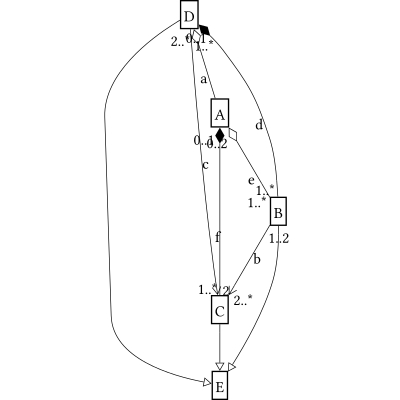
\includegraphics[min width=0.4\textwidth=0.6\textwidth,min height=0.4\textwidth=0.6\textwidth,keepaspectratio,max width=0.9\textwidth,max height=0.9\textwidth]{56/cdda6a11549572837c138bba9a1c158456881717bc6d103466234eed613892341d11af83b04c596701db35357ce8aed00a3a92e08161.pdf}\end{centering}



and the following object diagram (which conforms to it):



\begin{centering}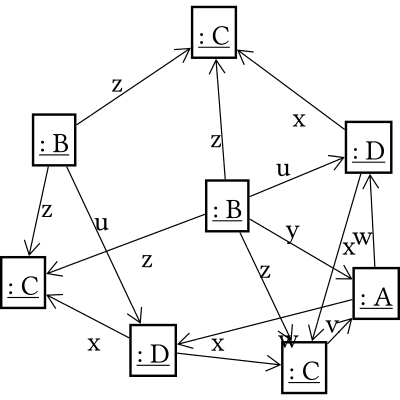
\includegraphics[min width=0.4\textwidth=0.6\textwidth,min height=0.4\textwidth=0.6\textwidth,keepaspectratio,max width=0.9\textwidth,max height=0.9\textwidth]{56/od3175862b30d91dbf6f4cd4e63838eb8da4661f8ad659a52a837e1e36d155f90210.pdf}\end{centering}



Which relationship in the class diagram (CD) corresponds to which of the links in the object diagram (OD)? 
 State your answer by giving a mapping of relationships in the CD to links in the OD. 
 To state that a in the CD corresponds to x in the OD and b in the CD corresponds to y in the OD, write the mapping as:\begin{verbatim}[(a,x),(b,y)]\end{verbatim}

Please note: Links are already grouped correctly and fully, i.e., all links with the same name (and only links with the same name!) in the OD correspond to exactly the same relationship name in the CD.

Thus, no relationship or link name should occur more than once in your mapping.

Please note: Classes are represented simplified here. 
 That means they consist of a single box containing only the class name but no sections for attributes or methods. 
 Nevertheless you should treat these simplified class representations as valid classes.

As navigation directions are used, please note that aggregations and compositions are only navigable from the ``part'' toward the ``whole'', i.e., they are not navigable in the opposite direction!

Please note: When hovering over or clicking on edges / nodes or their labels, the respective components that belong together are highlighted.

